\chapter{Environment configuration} \label{chr:envSetup}

This chapter describes the environment configuration needed to conduct the W-L test and the LA analysis, including an example of the linear accelerator setup from the National Institute of Oncology in Kraków. Images generated by the described linac will be used in later chapters.

\section{Configuration of environment for W-L test}

\begin{enumerate}
    \item A small BB phantom ($\phi$ around 3 $mm$), made of material with a high atomic number (typically steel, titanium or tungsten) is placed on the top of the couch and positioned at the mechanical isocenter determined by the treatment room laser system.

    \item The radiation beam is collimated to a perpendicular or cylindrical shape by the MLC, thereby ensuring that its centre coincides with the collimator axis and thus also passes through the mechanical isocenter.

    \item EPID is positioned on the opposite side of the BB so that the beam from the collimator falls on it.

    \item Number of images are generated for different combinations of gantry, collimator and couch angles. All angles need to be saved as metadata as it is needed by the algorithm.

    \item The resulting images can then be analyzed to identify any deviations from the norm, specifically when the shadow cast by the phantom is not located in the centre of the radiation field. \cite{wl_test_setup}

\end{enumerate}

\begin{figure}[H]
    \centering
    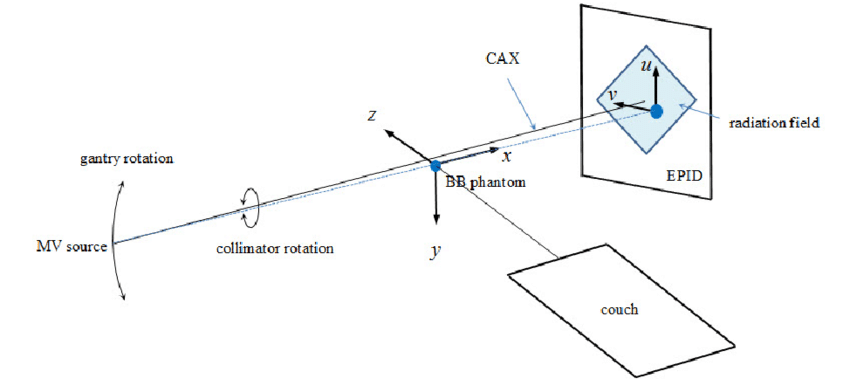
\includegraphics[width=0.8\textwidth]{Content/Images/wl_setup.png}
    \caption{Visualisation of W-L test environment configuration} \cite{wl_test_setup_image}
\end{figure}

\section{Configuration of environment for LA analysis}

The EPID is positioned in such a way that the radiation field is fully contained within it. In the LA analysis, the angles of the gantry, couch or collimator do not matter, however for the algorithm to work correctly, the photo must be arranged so that the leaves move horizontally, along the lower and upper edges of the resulting image. Nevertheless, the photo can be pre-processed and arranged correctly using digital techniques. The metadata that needs to be recorded are the planned leaf positions and the dimensions of the resulting image. 

Images taken in the W-L test configuration may be used for the LA test if they meet the above requirements.

\begin{figure}[H]
    \centering
    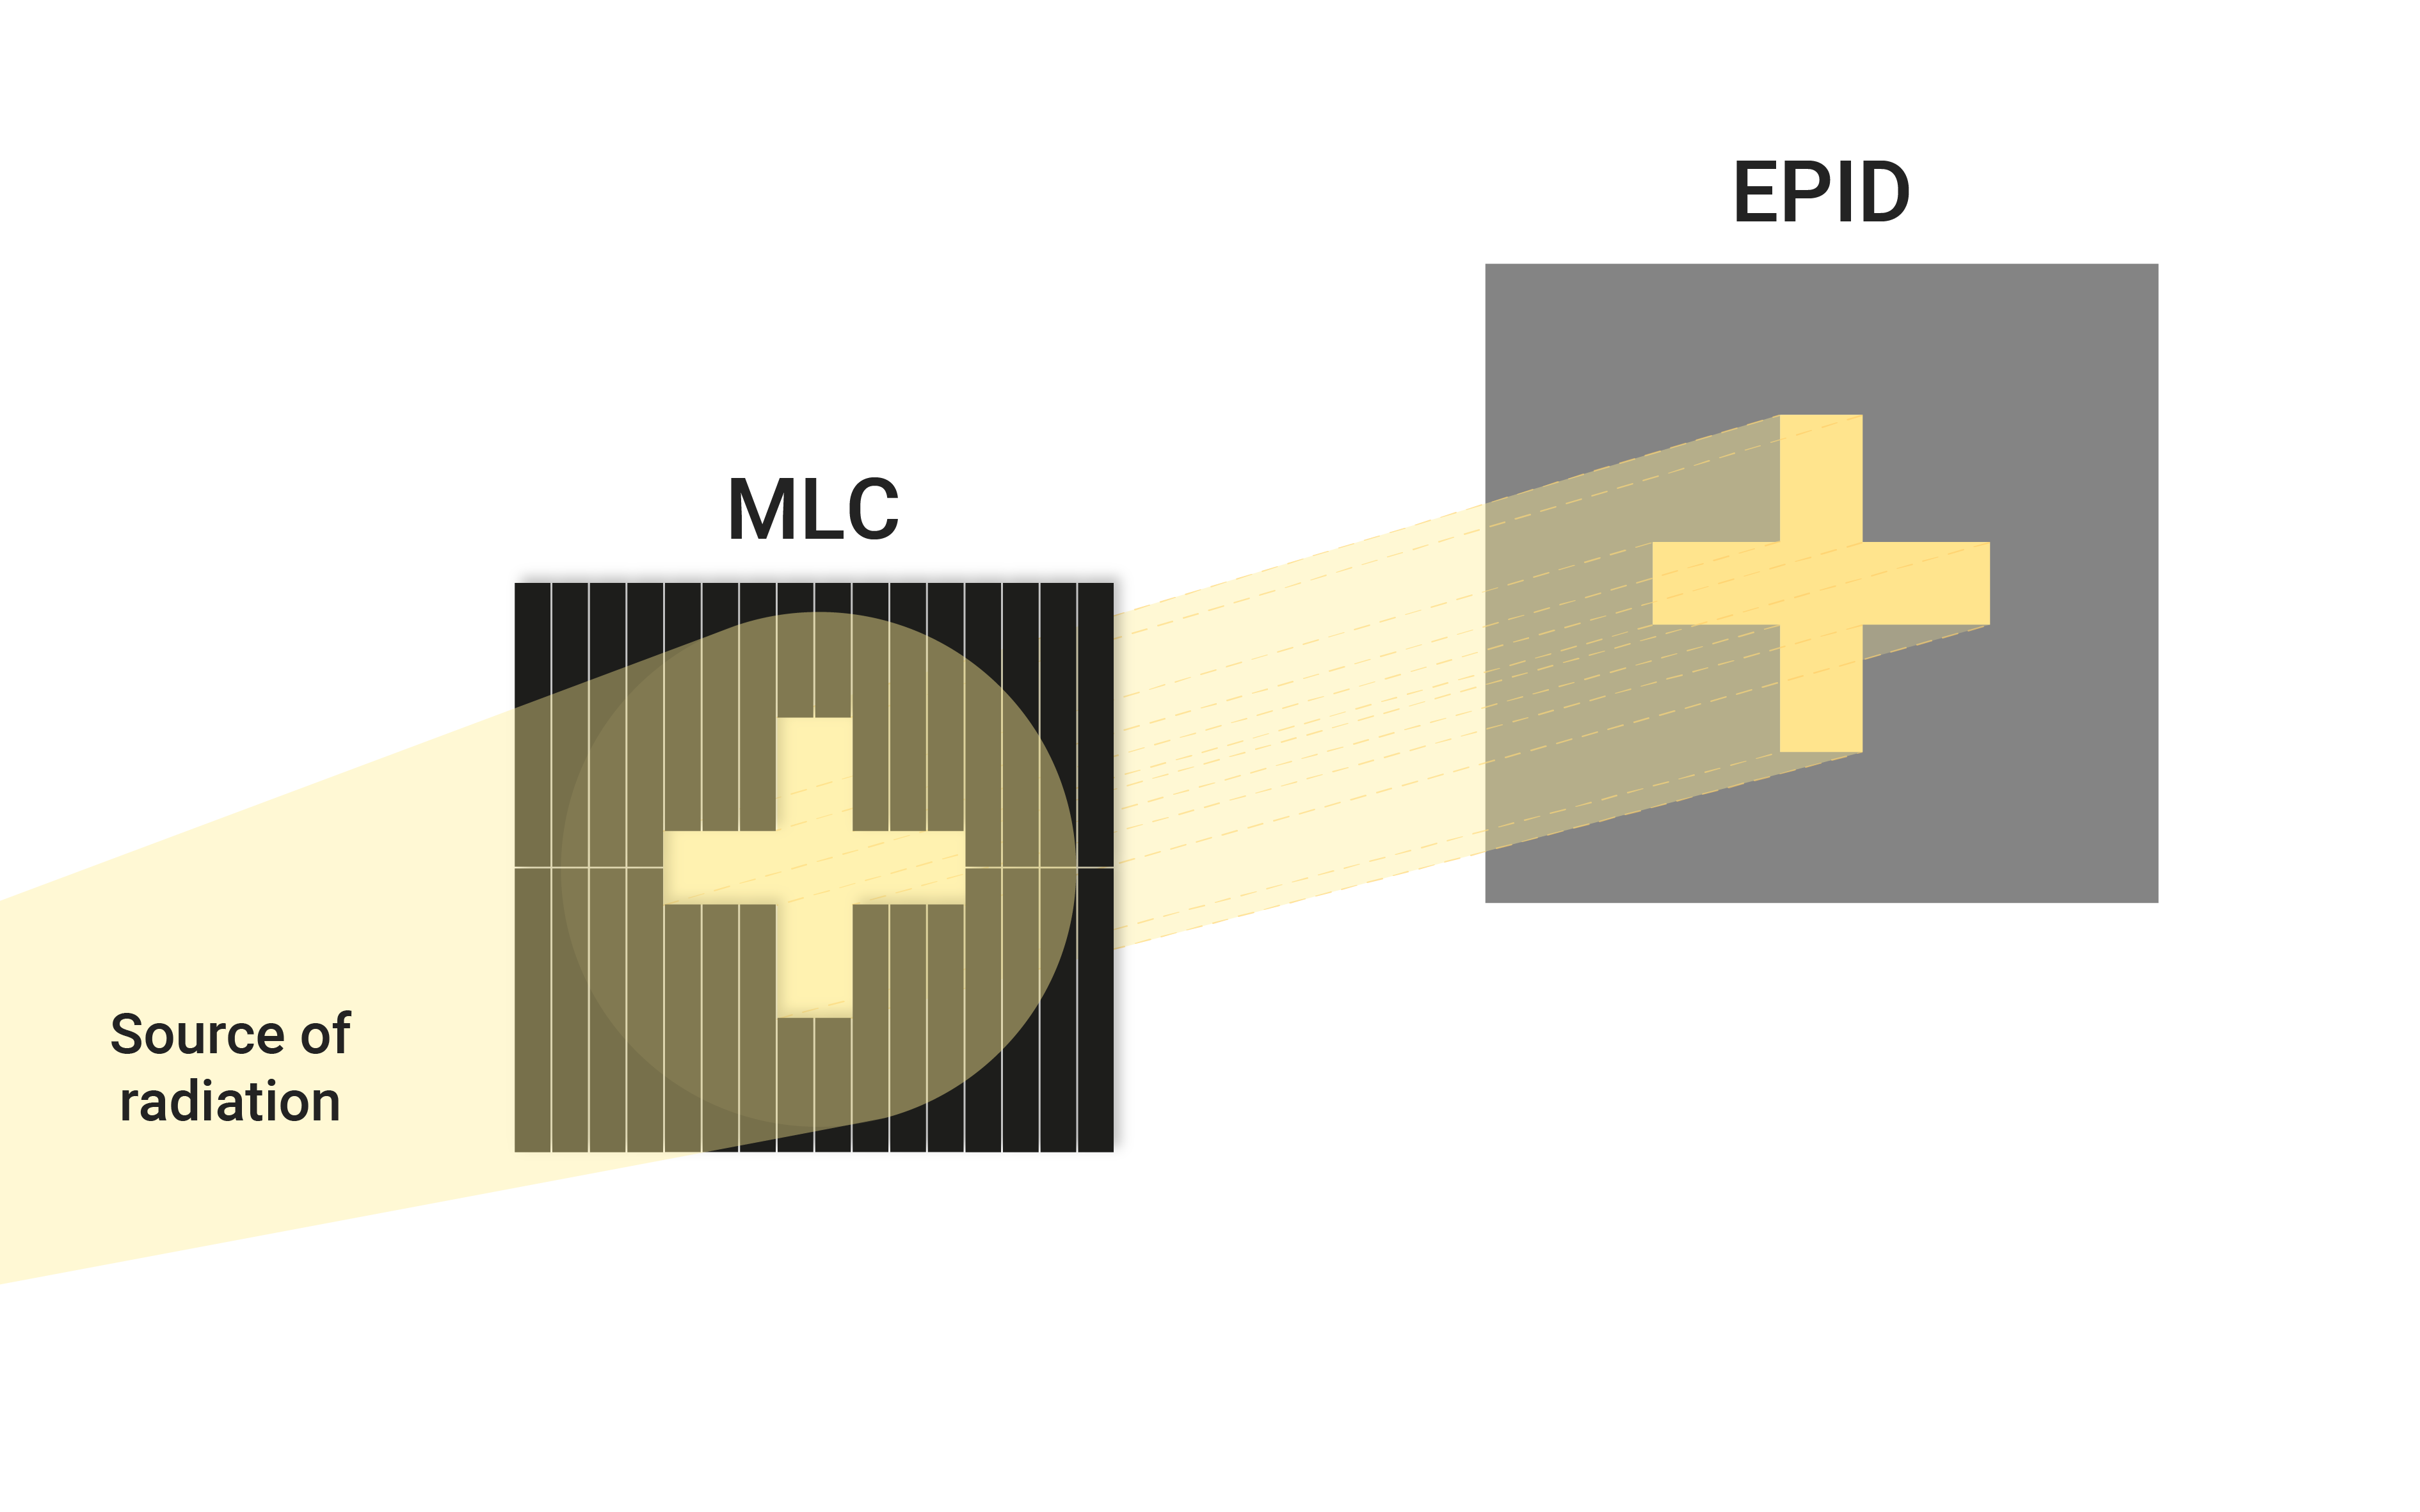
\includegraphics[width=0.85\textwidth]{Content/Images/LA_visualisation.png}
    \caption{Visualisation of LA analysis environment configuration}
\end{figure}


\section{Example of linac configuration from the National Institute of Oncology in Kraków} \label{sec:envSetupOncologyKrakow}

The accelerator used is Varian TrueBeam \cite{true_beam}. 
BB with a diameter of 2mm was placed in fixed on top of the coach and positioned using room laser system - \autoref{fig:nio_laser}.
EPID was positioned on the opposite side of the BB from the collimator - \autoref{fig:nio_epid}.
The leaves in the MLC have been formed so that the radiation field created by the radiation beam is a straight line with a square with a side of 10mm in the middle - \autoref{fig:nio_leaves}.

\begin{figure}[H]
    \centering
    \includegraphics[width=1\textwidth]{Content/Images/nio_epid.jpg}
    \caption{Setup of Varian TrueBeam linac}
    \label{fig:nio_epid}
\end{figure}

\begin{figure}[H]
    \centering
    \begin{subfigure}[b]{0.49\textwidth}
        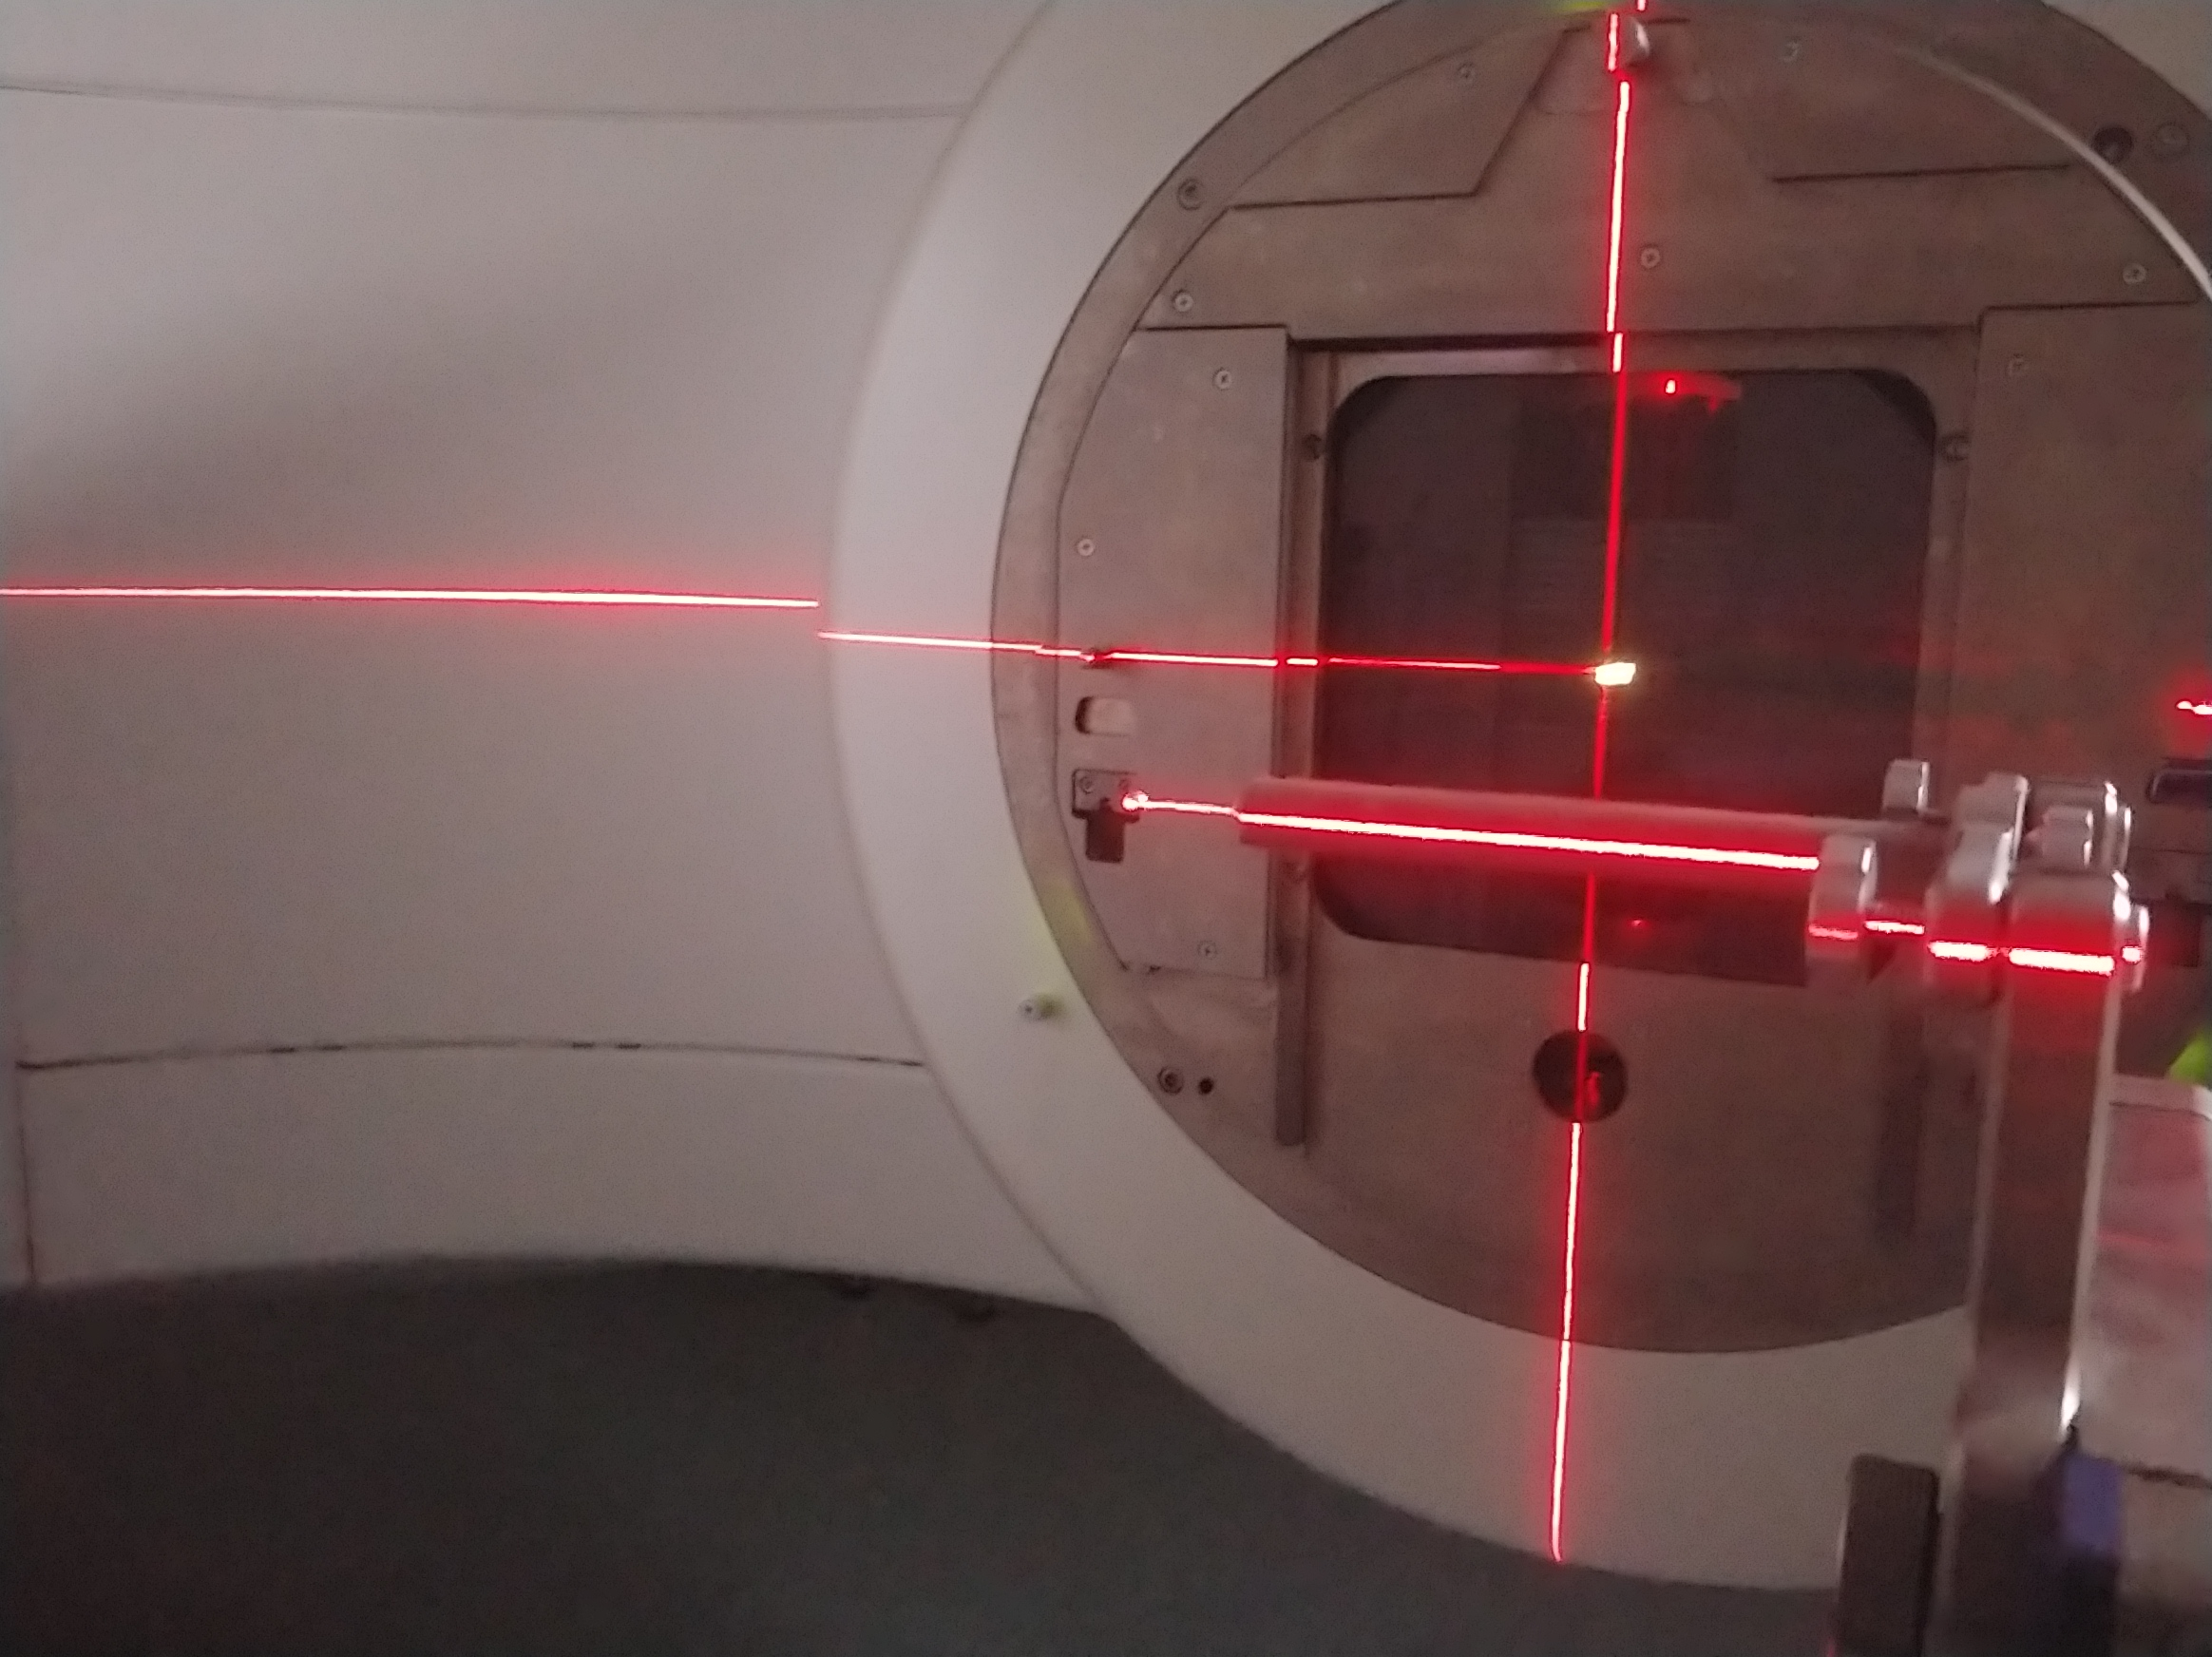
\includegraphics[width=\textwidth]{Content/Images/nio_laser.jpg}
        \caption{Positioning of BB using laser system}
        \label{fig:nio_laser}
    \end{subfigure}
    \begin{subfigure}[b]{0.49\textwidth}
        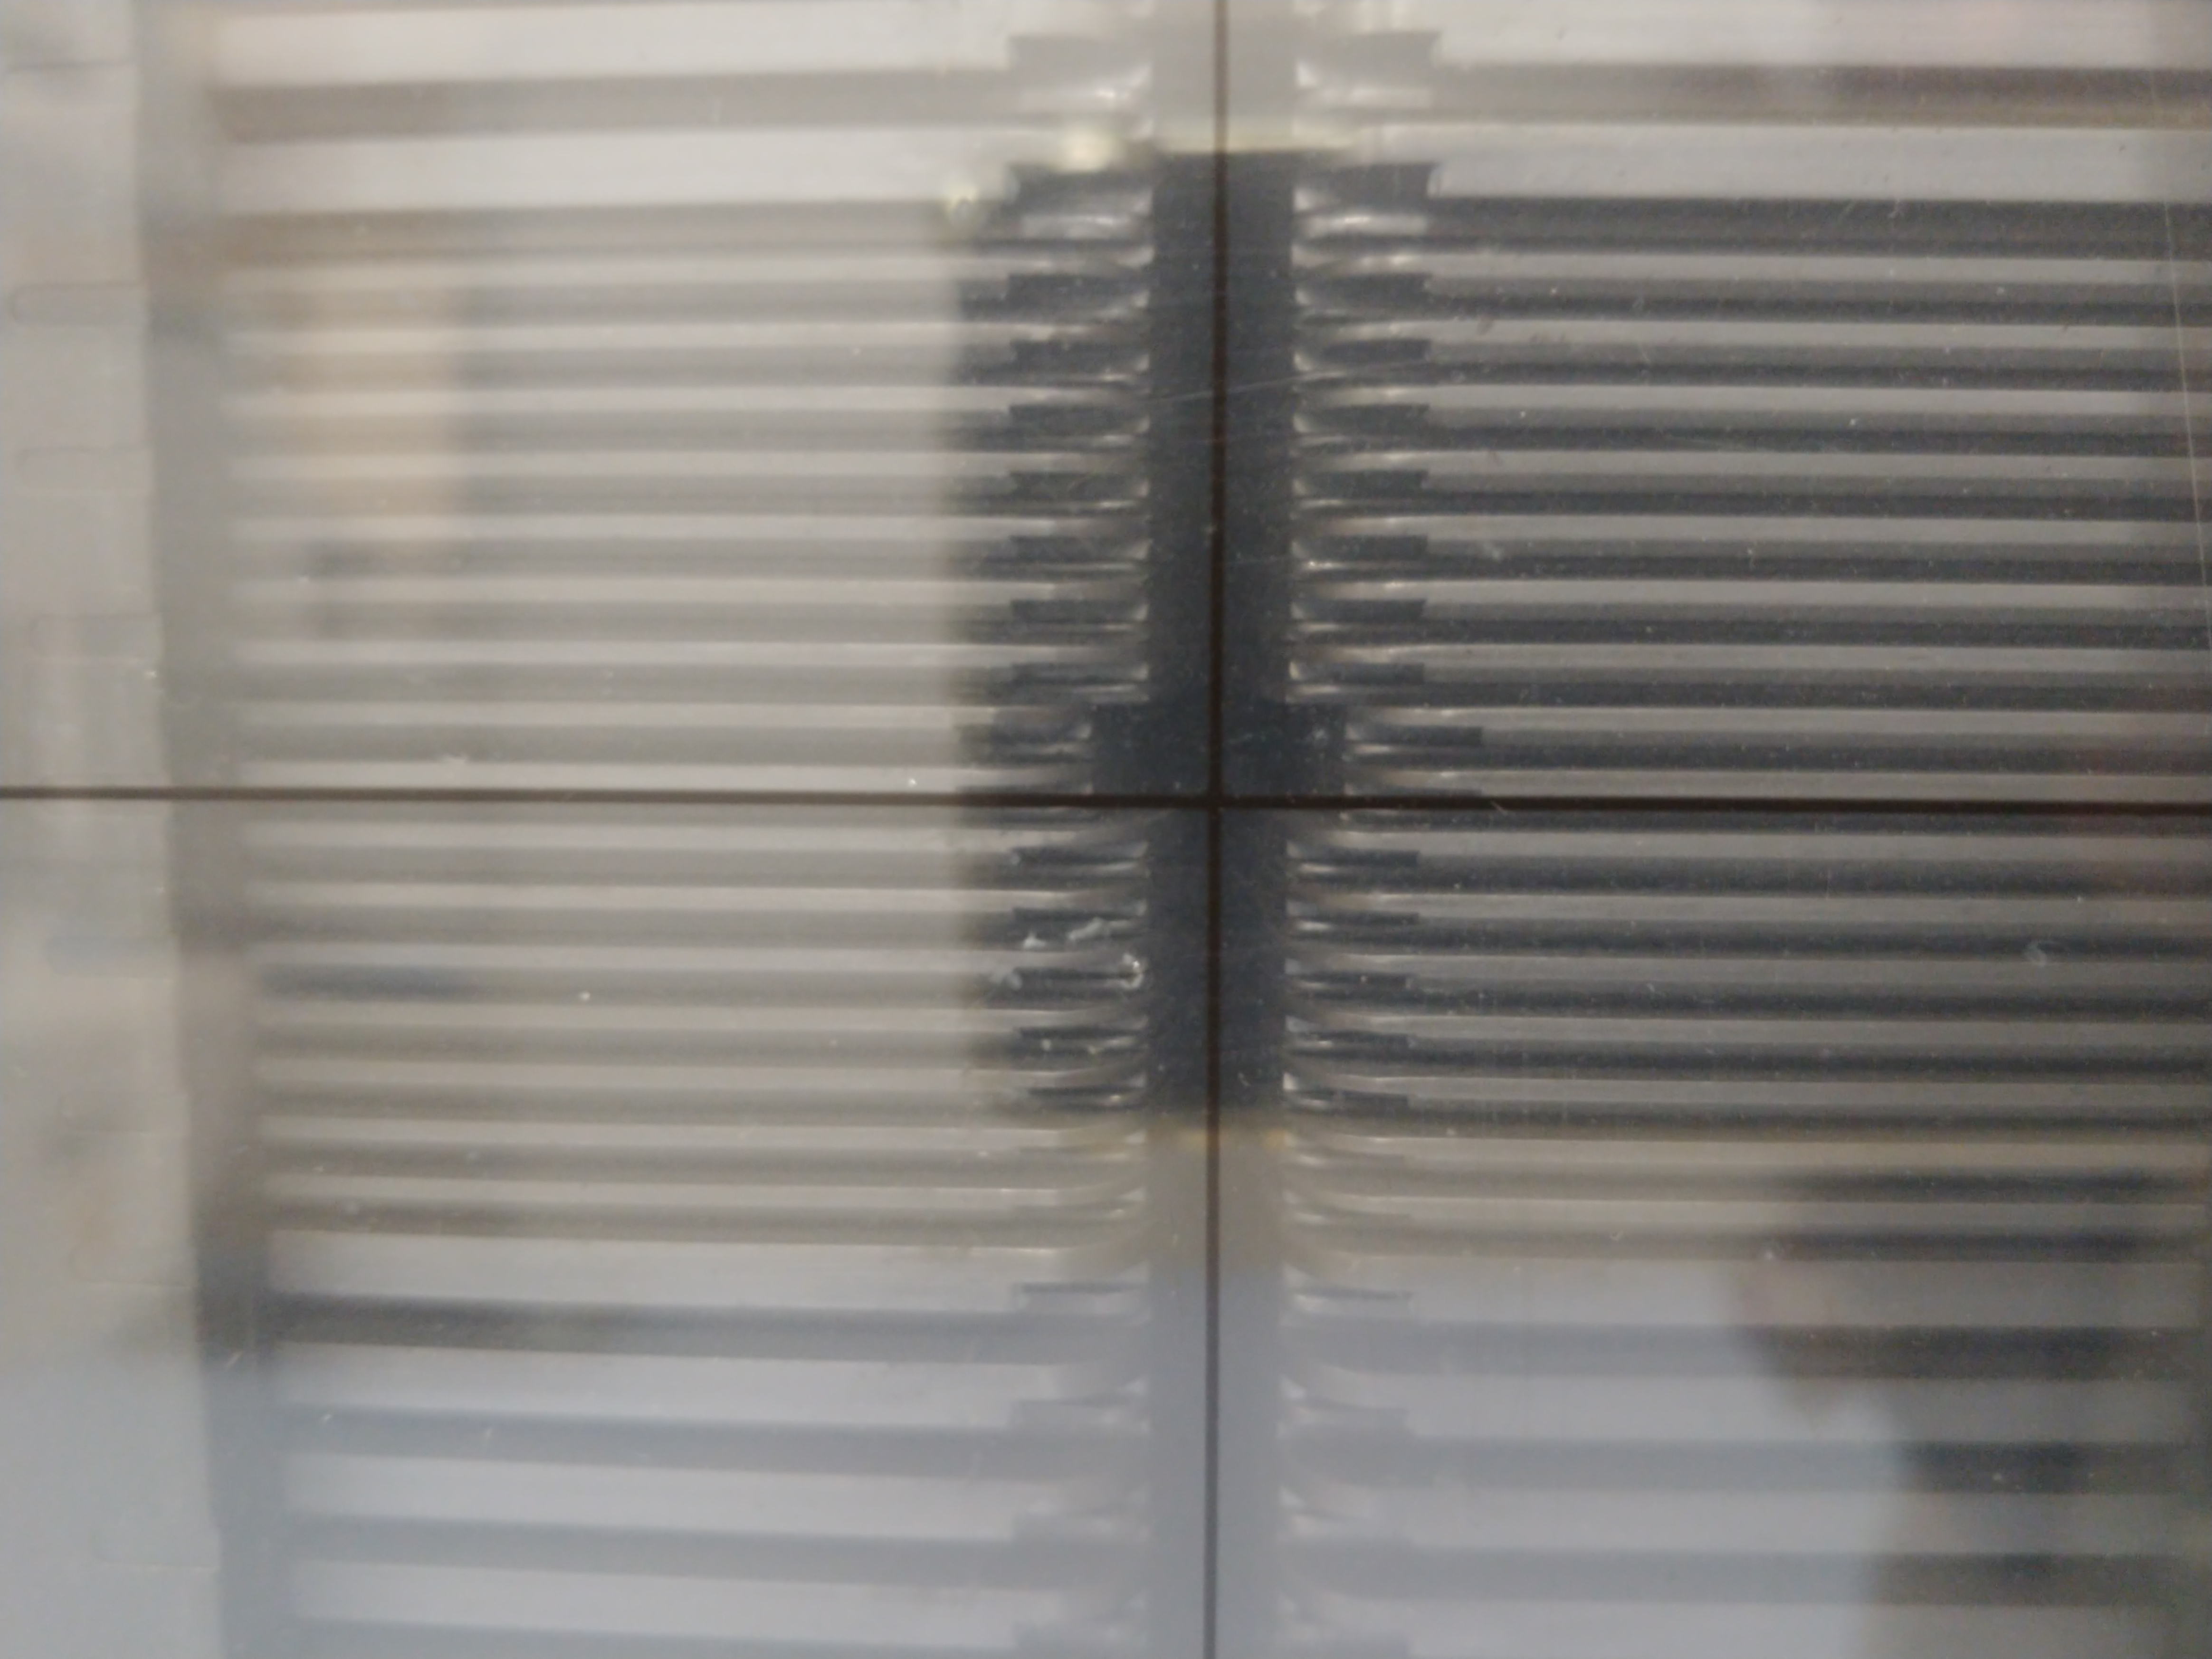
\includegraphics[width=\textwidth]{Content/Images/nio_leaves.jpg}
        \caption{Layout of leaves in MLC}
        \label{fig:nio_leaves}
    \end{subfigure}
\end{figure}